\documentclass[aspectratio=169,t]{beamer}

% Text encoding
% \usepackage{inputenc}
% \inputencoding{utf8}

% Language
%\usepackage{babel}
%\selectlanguage{english}

% Hyperlinks
\usepackage{hyperref}
\hypersetup{
  colorlinks=true,
  filecolor=magenta,
  urlcolor=cyan,
  citecolor=cyan,
  linkcolor=cyan
}

% Tables
\usepackage{booktabs}

% Math
\usepackage{amsmath}
\usepackage{amssymb}
\usepackage{bm}
\usepackage{siunitx}
\usepackage{mathtools}

% Unnumbered footnote
\let\svthefootnote\thefootnote%
\textheight 1in
\newcommand\blankfootnote[1]{%
  \let\thefootnote\relax\footnotetext{#1}%
  \let\thefootnote\svthefootnote%
}

% Tikz
\usepackage{tikz}
\usetikzlibrary{positioning}

% References
%\usepackage[natbib=true]{biblatex}
%\addbibresource{references.bib}
%\usepackage{natbib}

% Presentation settings
\mode<presentation>
{
  \usetheme{default}
  \usecolortheme{default}
  \usefonttheme{default}
  \setbeamertemplate{caption}

  % Theme hacking
  %% Default margin: 1cm
  \setbeamersize{text margin left=0.5cm, text margin right=0.5cm}

  %% Footer
  \setbeamerfont{footline}{size=\fontsize{3}{0}\selectfont}
  \setbeamercolor{section in head/foot}{fg=white, bg=ISUcardinal}
  %%% https://tex.stackexchange.com/a/111466/225233
  \setbeamertemplate{footline}
  {
    \hypersetup{allcolors=.}
    \leavevmode%
    \hbox{%
      \begin{beamercolorbox}[wd=.2\paperwidth,ht=2.25ex,dp=1ex,left]{section
          in head/foot}%
        \usebeamerfont{author in head/foot}\insertshortauthor{}
      \end{beamercolorbox}%
      \begin{beamercolorbox}[wd=.6\paperwidth,ht=2.25ex,dp=1ex,center]{section
          in head/foot}%
          \usebeamerfont{title in head/foot}\insertshorttitle{}
        % \usebeamerfont{title in head/foot}Automatic Dynamic
        % Relevance Determination
      \end{beamercolorbox}%
      \begin{beamercolorbox}[wd=.2\paperwidth,ht=2.25ex,dp=1ex,right]{section
          in head/foot}%
        \usebeamerfont{date in head/foot}\insertshortdate{}\hspace*{2em}
        \insertframenumber{} / \inserttotalframenumber\hspace*{2ex}
      \end{beamercolorbox}}%
    \vskip0pt%
  }

  %% Hide navigation bar
  \beamertemplatenavigationsymbolsempty{}

  %% ISU colors
  \definecolor{ISUcardinal}{RGB}{200,16,46}
  \definecolor{ISUgold}{RGB}{241,190,72}
  \definecolor{ISUgray}{RGB}{82,71,39}
  \definecolor{ISUsand}{RGB}{155,148,95}
  \definecolor{ISUgreen}{RGB}{202,199,167}

  %% Title page
  \setbeamercolor*{title}{fg=ISUcardinal}

  %% Frame
  \setbeamercolor{frametitle}{fg=white, bg=ISUcardinal}

  %% Lists
  \setbeamertemplate{itemize item}[square]
  \setbeamertemplate{itemize subitem}[triangle]
  \setbeamertemplate{itemize subsubitem}[triangle]

  \setbeamercolor{itemize item}{fg=ISUcardinal}
  \setbeamercolor{itemize subitem}{fg=ISUcardinal}
  \setbeamercolor{itemize subsubitem}{fg=ISUcardinal}

  \setbeamercolor{description item}{fg=ISUcardinal}

  %\setlength{\leftmargini}{0pt}
  \setlength{\leftmarginii}{10pt}
}

\usepackage{DejaVuSerif}
\usepackage[T1]{fontenc}

% Setup
\graphicspath{{include/}}

\title{\textbf{Automatic Dynamic Relevance Determination} \\ of
  atmospheric states over vertical pressure grids \\ for the MLS
  forward model emulation}

\author[Damiano, Niemi]{
  \textbf{Luis Damiano}\footnote{
    \tiny{\href{mailto:ldamiano@iastate.edu}{ldamiano@iastate.edu}}
  }, Jarad Niemi}

\institute{Department of Statistics \\ Iowa State University}

\date[October 14, 2021]{\tiny{NASA JPL Uncertainty Quantification for
Remote Sensing Inverse Problems
Virtual Breakout Meeting}\\ October 14, 2021}

\begin{document}

% Title page
\begin{frame}
  \titlepage{}
  % \vspace{0.1in}
  {
    \tiny{
      Funded, in part, by
      \begin{itemize}
      \item[-] ISU Presidential Interdisciplinary
        Research Initiative on C-CHANGE:~Science for a Changing
        Agriculture
      \item[-] Foundation for Food and Agriculture Research
      \end{itemize}
    }
  }
\end{frame}

% Introduction -----------------------------------------------------------------
\begin{frame}
  \frametitle{The data}
% 3.15.cm
  \begin{figure}[h!]
    \centering
    \includegraphics<2>[height=4.15cm]{plot-input-examples-selected-0.png}%
    \includegraphics<3>[height=4.15cm]{plot-input-examples-selected-1.png}%
    \includegraphics<4>[height=4.15cm]{plot-input-examples-selected-2.png}%
    \includegraphics<5-6>[height=4.15cm]{plot-input-examples-selected-3.png}
  \end{figure}

  \only<1-5>{
    \begin{description}[labelwidth=117]
    \item[Index vector]<2-> $\mathbf{t}$ with the vertical pressure level
    \item[State vector]<3-> $\mathbf{x}_i$ characterizing an atmospheric
      vertical profile
    \item[Output scalar]<4-> $y_i \in [0, 1]$ is the radiance first
      functional principal component~\cite{johnson2020}
    \item[Sounding]<5-> a collection of an observed radiance, retrieved
      state and pressure vectors
    \end{description}
  }

  \only<6>{
    \vfill
    \begin{center}
      \definecolor{bright-spark}{RGB}{255, 195, 59}
      \tikzstyle{nice-rectangle} = [rectangle, rounded corners,
      minimum width=3cm, minimum height=1cm, text centered,
      draw=ISUcardinal, fill=bright-spark, font=\sffamily]

      \begin{tikzpicture}
        % We start by placing the blocks
        \node (input) [nice-rectangle] {Functional input}; \node
        (output) [nice-rectangle, right=of input] {Scalar output};
        \draw [->] (input) [above] -- node {$f$} (output);
      \end{tikzpicture}
    \end{center}
    \vfill
  }

\end{frame}

\begin{frame}{Functional Input Gaussian Process (fiGP)}
  \begin{align}
    \mathbf{y}
    &\sim \mathcal{N}\left(0, \sigma_{f}^{2} \ \mathbf{R}_f + \sigma_{\varepsilon}^{2}\mathbf{I}\right) \\
    {\left(\mathbf{R}_f\right)}_{ij}
    &=
      \text{exp}\left\{
      -0.5 \theta^{-2} \ d_f(X_i, X_j)
      \right\} \\
    \invisible<1>{
    d_f(X_i, X_j)
    &= \int_{\mathcal{T}}
      \omega(t)
      {\left(X_i(t) - X_j(t) \right)}^2 dt
      }
  \end{align}

  \blankfootnote{
    $\sigma_{\varepsilon}^2 > 0$,
    $\sigma_{f}^2 > 0$,
    $\theta > 0$,
    $i, j = 1, \dots, N$
  }
  \blankfootnote{
    \invisible<1>{
      $\omega(t): \mathcal{T} \to (0, \infty)$
    }
  }

  \begin{description}
  \item[Multiple inputs]<3-> e.g., correlation product
  \item[Complex index spaces]<4-> e.g., spatio-temporal structures
  \item[Flexibility]<5-> no need to match input-output structure nor index space
  \end{description}
\end{frame}


% \begin{frame}
%   \frametitle{A flexible weight function}

%   \begin{figure}[h!]
%     \centering
%     \includegraphics[width=.7\textwidth]{plot-weight-functions}
%   \end{figure}
%   \begin{align*}
%     \omega(t)
%     &= \text{exp}\left\{-(t - \tau) \lambda \kappa^s s\right\} \\
%     s
%     &= \text{sign}(t - \tau) \\
%     \lambda &> 0 \\
%     \tau &\in [0, 1] \\
%     \kappa &> 0
%   \end{align*}

%   \blankfootnote{A generalization of~\cite{morris2012}}
% \end{frame}

\begin{frame}
  \frametitle{Trapezoidal approximation}

  \begin{figure}[h!]
    \centering
    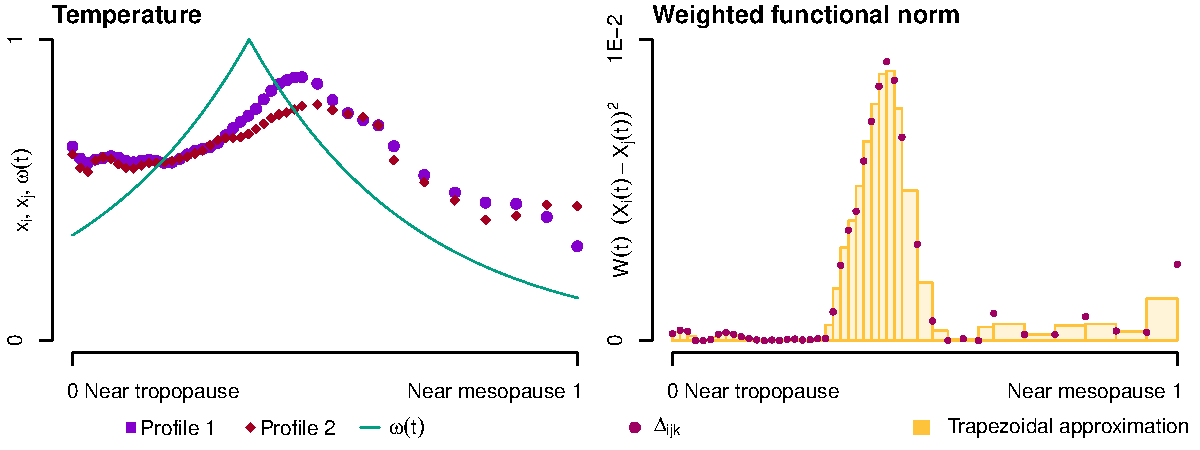
\includegraphics[width=.6\textwidth]{plot-trapezoidal-approx}
    \caption[]{Trapezoidal approximation}
  \end{figure}

  {
    \setlength{\abovedisplayskip}{-1cm}
    \begin{align}
      \int_{\mathcal{T}}
      \omega(t)
      {\left(X_i(t) - X_j(t) \right)}^2 dt
      \approx
      &
        \sum_{k = 2}^{K} {
        \left(t_{k} - t_{k - 1}\right)
        \frac{
        \Delta_{i, j, k} +
        \Delta_{i, j, k - 1}
        }{2}
        } \\
      \Delta_{i, j, k} =
      & \
        \omega(t_{k-1}) {\left(x_{i, k} - x_{j, k}\right)}^2
    \end{align}
  }

  \blankfootnote{See~\cite{muehlenstaedt2017a} for a B-spline
    approach}
\end{frame}

% Results ----------------------------------------------------------------------
% \begin{frame}
%   \frametitle{fiGP:~an implementation}
%   \begin{itemize}
%   \item 1,000 soundings
%   \item Nine model configurations
%   \item One model fit separately per input
%   \item Fully Bayesian inference
%   \item Hamiltonian Monte Carlo using Stan
%   \item 16 chains
%   \item 500 post-warmup iterations
%   \item 8,000 posterior samples total
%   \item About 3 hours at 2 teraflops (18 total with warmup)
%   % 3 nodes x 2 sockets x 8 cores x 2.6ghz x 16 FLOPS/clock
%   \end{itemize}
% \end{frame}

\begin{frame}
  \frametitle{Weight function posterior samples}

  \begin{figure}
    \centering
    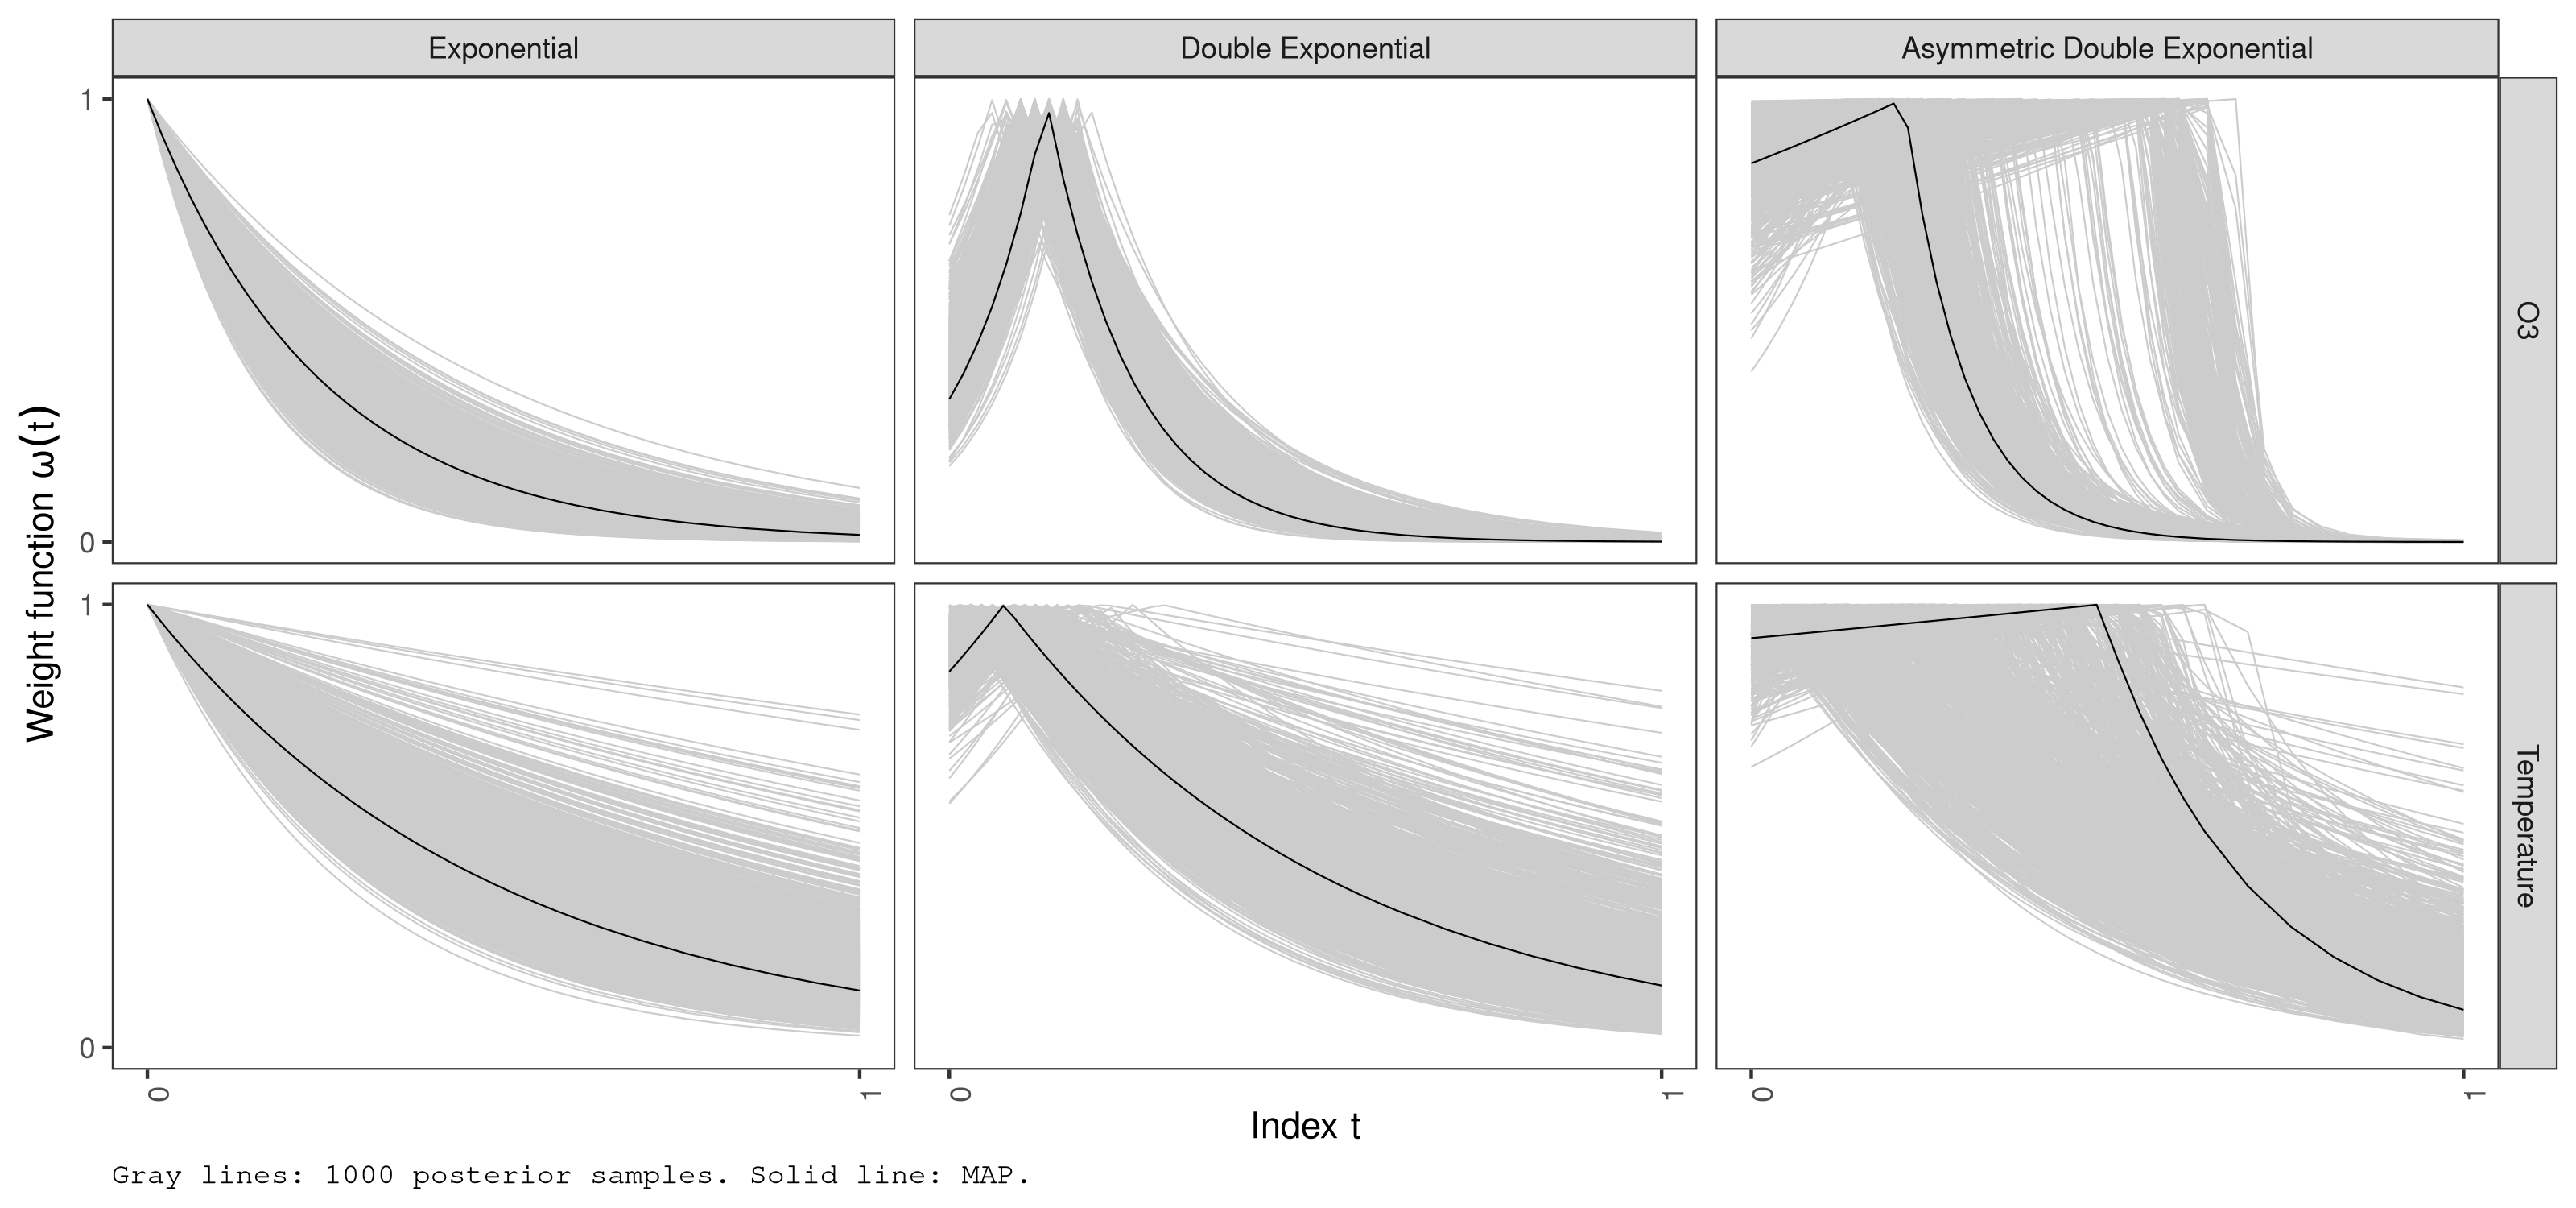
\includegraphics[width=1\textwidth]{fit-full-posterior-weights-selected.png}
  \end{figure}
\end{frame}

\begin{frame}
  \frametitle{Cross-validation overview}

  \begin{figure}
    \centering
    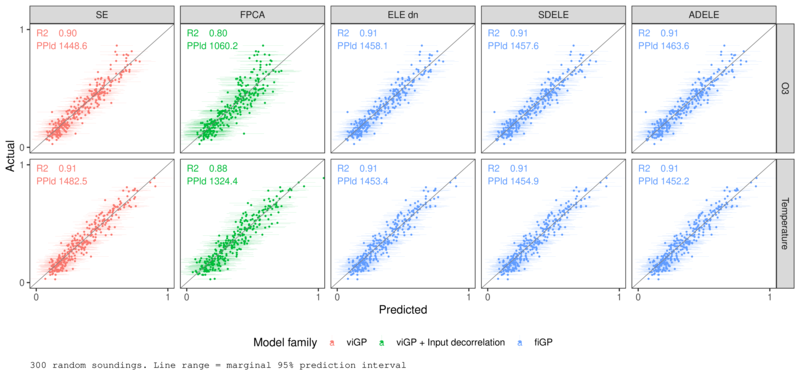
\includegraphics[width=1\textwidth]{xvalidation-actual-predicted-scatterplot-selected}
  \end{figure}
\end{frame}

\begin{frame}
  \frametitle{Learnings from this lil' experiment}

  \small

  \begin{columns}[t]
    \begin{column}{.45\textwidth}
      Vector input GP
      \begin{itemize}
      \item[+]<2-> Well-known, well-tested, readily available software
      \item[+]<2-> Many fast approximations available
      \item[+]<3-> Missing data in inputs
      \end{itemize}
      \vspace{0.25cm}
      \begin{itemize}
      \item[-]<3-> Output-agnostic FPCA decisions%: smoother, bases, knots
      \item[-]<3-> Potential loss of information if not retaining all
        components
      \item[-]<4-> Interpretation
      \item[-]<5-> Parameter space scales with
        functional input resolution
      \end{itemize}
    \end{column}

    \begin{column}{.45\textwidth}
      Functional input GP
      \begin{itemize}
      \item[+]<3-> Explicit link output correlation and
        input functional structure
      \item[+]<3-> Domain-specific knowledge
      \item[+]<4-> Interpretation
      \item[+]<5-> Parsimony
      \item[+]<6-> \alert{\textbf{Complex index spaces}},
        e.g., spatio-temporal inputs
      \end{itemize}
      \vspace{0.25cm}
      \begin{itemize}
      \item[-]<2-> Custom software
      \item[-]<2-> A less-explored approach, further research needed
      \end{itemize}
    \end{column}
  \end{columns}

\end{frame}

% References -------------------------------------------------------------------
\section{References}

\begin{frame}{References}
  \tiny
  \bibliographystyle{unsrt}
  \bibliography{references}
\end{frame}

\end{document}

%%% Local Variables:
%%% mode: latex
%%% TeX-master: t
%%% End:
